\chapter{\IfLanguageName{dutch}{Stand van zaken}{State of the art}}
\label{ch:stand-van-zaken}
Dit deel begint met een inleiding over virtualisatie, de reden om virtualisatie te doen en de verschillende soorten. Hiervoor worden eerst Virtuele machines en Hypervisors besproken. Gevolgd door een geschiedenis en ontstaan van container virtualisatie en de  effectieve werking van ervan. Om vervolgens een vergelijking tussen Virtuele machines en Container virtualisatie te schetsen. Dit deel wordt afgesloten met het overlopen van de gevonden aanbieders van software voor container virtualisatie de zouden kunnen worden getest.

% Tip: Begin elk hoofdstuk met een paragraaf inleiding die beschrijft hoe
% dit hoofdstuk past binnen het geheel van de bachelorproef. Geef in het
% bijzonder aan wat de link is met het vorige en volgende hoofdstuk.

% Pas na deze inleidende paragraaf komt de eerste sectiehoofding.
\section{Wat is virtualisatie}

Virtualisatie is in essentie het maken van een abstractie van de onderliggende hardware waarop  software berust tijdens het uitvoeren van processen. Naast de hardware laat virtualisatie ook toe om het besturingssysteem waarmee de software de hardware aanspreekt naar de hand te zetten. Een eerste reden om aan virtualisatie te doen is om mogelijke verschillen in hardware en besturingssystemen uit te sluiten.  Software dat ontwikkeld wordt in een omgeving met zekere hardware en besturingssysteem kan zich anders gedragen of zelfs incompatibel zijn met de omgeving waarin de software effectief in productie gebruikt  moet worden. Een verder voordeel dat virtualisatie toelaat is een betere benutting van hardware, zeker bij servers. De fysieke hardware van een server kan door middel van virtualisatie  gebruikt worden om meerdere applicaties draaien die elk andere vereisten hebben. Ook hier help de abstractie van de oorspronkelijke hardware en eventuele besturingssysteem van de server een gebruiker die software wilt draaien op een server om dit te kunnen zonder de hardware van de server te moeten kennen \Autocite{Yadav2018,Jangla2018}.

Voor virtualisatie bestaan er verschillende manieren van aanpak. Een eerste is de virtuele machine manier wat in volgend deel besproken wordt. En tweede manier is van gedachte om de virtualisatie van software te kunnen beheren  op analoge wijze als Vrachtcontainers. Ten derde is er ook nog emulatie, een vorm van virtualisatie die niet verder behandeld wordt in deze thesis.

\section{Virtuele machines en Hypervisors}

\subsection{Virtuele machines}
Een eerste manier van virtualisatie is een volledige Virtuele Machine (VM). Bij VM wordt er virtuele hardware voorzien van een eigen besturingssysteem. Aan de hand van dit besturingssysteem en de virtuele hardware is het dan ook mogelijk om in deze VM een applicatie te draaien alsof hij op een echte machine staat. Verder zorgt deze virtualisatie ervoor dat het draaien van een applicatie in een VM volledig hetzelfde zal blijven zou de VM zelf op andere hardware berusten. Het besturingssysteem dat in de VM draait is volledig configureerbaar waardoor het mogelijk is om andere soorten toestellen na te bootsen, zoals een gsm. Een VM zelf is niets meer dan de ruimte op de opslag schijf die het gebruikt voor zijn eigen instellingen en zijn eigen interne bestanden te bewaren. Wegens de aanwezigheid van een volledige besturingssysteem kan de geheugenruimte die een VM inneemt groot. Het direct aanspreken van bestanden in het interne geheugen van een VM langst buitenaf zonder via de VM’s kanalen te werken is ook standaard niet mogelijk\autocite{Eder2016}.

\subsection{Hypervisors}

Omdat een VM beschouwd kan worden als gewoon een deel van het geheugen dat gebruikt wordt om het op te slaan is er nood aan bijkomende software om de VM effectief bruikbaar te maken. Deze bijkomende software wordt een Hypervisor genoemd. De Hypervisor staat voornamelijk in voor het vertalen van input die de VM naar zijn eigen virtuele hardware stuurt te vertalen en om te zetten zodat ze door de werkelijke hardware uitgevoerd kunnen worden. De virtuele kernel van de VM dus dankzij de hypervisor effectief uitgevoerd. Een Hypervisor blijft niet bij het beheren van maar één VM, het laat ook toe om nieuwe VM’s aan te maken door middel van het alloceren van geheugenruimte en de virtuele hardware voor te bereiden om een besturingssysteem op te zetten. Aansluiten laat de Hypervisor dan ook toe dat er meerdere VM’s tegelijkertijd in gebruik kunnen worden genomen.  Vaak laat een hypervisor ook toe om op een eenvoudige manier de VM van buitenaf te bereiken. Hetzij via een bestand locatie te organiseren die je zowel via de VM als van buiten af kunt bereiken of het klaarzetten van virtuele netwerken waarmee de VM’s onderling of naar buiten kunnen communiceren.

Onder Hypervisors zijn er twee verschillende  types te onderscheiden. Type 1 Hypervisors staan zelf direct op de hardware van de machine. Hierdoor heeft de hardware geen directe besturingssysteem, en spreekt de hypervisor direct de machine kernel aan voor de uitvoering van opdrachten. Zo zijn de  aanwezige besturingssystemen enkel deze die als gast door de Hypervisor in een VM worden uitgevoerd op de hardware. Type 2 Hypervisors daarentegen worden uitgevoerd als een gebruikers applicatie binnen een host besturingssysteem.  De VM’s draaien genest in een conventioneel besturingssysteem en omgeving die gebruikt kan worden. Het verschil tussen de twee wordt geïllustreerd in figuur \ref{fig:hyperviors} \autocite{Yadav2018,Eder2016}.

\begin{figure}[h]
    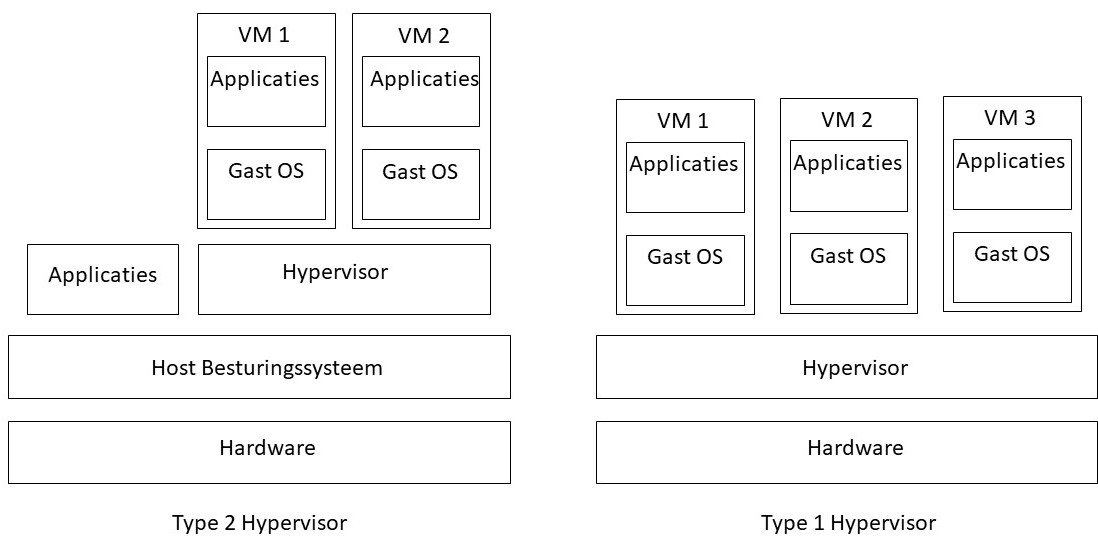
\includegraphics[width=\linewidth]{img/hypervisors.jpg}
    \caption[Verschil tussen type 1 en type 2 hypervisor]{Dit figuur toont het verschil tussen de locatie van de hypervisor en zijn VM’s ten opzichte van de hardware.}
    \label{fig:hyperviors}
    \centering
\end{figure}

\section{Container virtualisatie}

Bij container virtualisatie is de kerngedachte om enkel te virtualiseren wat de applicatie die effectief nodig heeft. De applicatie zelf en alle dependencies die het nodig heeft worden gebundeld in een ‘container’ die overal kan worden gebruikt. In deze vorm van virtualisatie wordt de hardware en besturingssysteem niet gevirtualiseerd, de containers spreken zelf het besturingssysteem van de host aan om procestijd en andere hardware middelen aan te spreken. Doordat het beeld, ook image genoemd, van een container minder bijhoud dan dat van een VM zijn ze kleiner en starten ze sneller op \autocite{Eder2016,Jangla2018}.

\subsection{Korte geschiedenis van container virtualisatie}

Een oudere manier van container virtualisatie bestaat al lang in de vorm van de \textbf{ch}ange \textbf{root} functionaliteit in unix gebaseerde besturingssystemen. Met Chroot is het sinds 1982 mogelijk om de root directory van proces, en zijn sub processen, aan te passen en zo te beperken  waartoe het proces toegang heeft. Vanuit chroot is het Linux containers (LXC) project\footnote{\url{https://linuxcontainers.org/}} gestart en werd het in 2008 mogelijk om Linux gebaseerde container virtualisatie te doen via de ontwikkelde toolkit. Met deze toolkit is het iets eenvoudiger om containers te maken maar is er nog veel kennis van de Linux kernel nodig\autocite{Eder2016,SenthilKumaran2017}.

In 2013 kwam Docker\footnote{\url{https://www.docker.com/}} op de markt en slaagde erin om het werken met Linux gebaseerde container veel te vereenvoudigen ten opzichte van LXC’s toolkit\autocite{Hykes2013}. Door Docker’s succes in het vereenvoudigen van de workflow voor het creëren en draaien van containers is de technologie dan ook in een versnelling terecht gekomen.  Een grote vernieuwingen die Docker zelf bracht was het werken met duidelijke container images voor het maken en bewaren van containers. Hierbij bied het ook de Docker hub aan om deze images te bewaren en te delen. Dockers succes werd verder ondersteunt doordat Google al zelf een tijd intern werkte met containers en zo geschikte software kon aanbieden om gebruiksvriendelijk  meerdere containers tegelijkertijd te beheren. In 2016 publiceerde Google een retrospectieve die uitgelegde hoe het al een aantal jaren met Linux gebaseerde containers werkte door middel van oudere software Borg en Omega, en hiermee Kubernetes{\url{https://kubernetes.io/}} ontwikkelde. De gebruiksvriendelijkheid en voordelen die de lichter virtualisatie kan bieden zorgden er dan ook voor dat container virtualisatie door velen werd geadopteerd \autocite{Eder2016}.

\subsection{Engine}

Voor het aanmaken en draaien van containers op een systeem is er nood aan een container manager of engine. Met een container engine is het mogelijk om een container image te draaien of aan de hand van een image meerdere containers van dezelfde applicatie te maken. Het effectief draaien van de container wordt gedaan aan de hand van een runtime dat vaak gebundeld zit in de engine de rest van de functionaliteiten is eigen aan de engine. De werking van containers word getoond in figuur \ref{fig:Containers}. De levenscyclus van een container te laten beheren door een engine begint met het ophalen van een container image om van te vertrekken. Deze kunnen gedownload worden van een publieke of privé repository van images. Dit vertrekpunt kan dan verder worden aangepast voor de specifieke applicatie noden vooraleer terug opgeslagen te worden in nieuwe image. Hierna kan de image worden gebruikt om een container te starten. op basis van een zelfde image kunnen gelijktijdig meerdere containers worden gestart. Containers hebben ook de mogelijkheid om data weg te schrijven naar een externe volume zodanig dat deze gegevens niet verloren gaan bij het stoppen van een container. Het beheren en toekennen van deze volumes behoort ook tot de functionaliteiten van een engine.Een container engine kan software zijn die on- premise geïnstalleerd is, waardoor de configuratie zelf te doen is, of het kan worden aangeboden door een Cloud service provider, zodat er in deze Cloud omgeving zonder te veel configuratie met containers kan worden gewerkt\autocite{Casalicchio2020}.
\begin{figure}[h]
    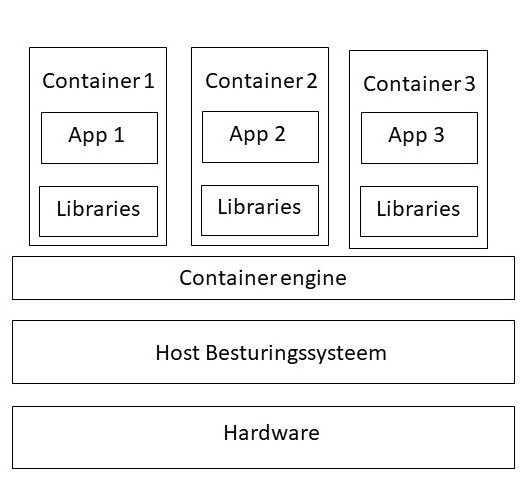
\includegraphics[width=\linewidth]{img/container.jpg}
    \caption[Schema container virtualisatie]{Een schematische voorstelling van container virtualisatie}
    \label{fig:Containers}
    \centering
\end{figure}

\subsection{Orchestration}
Om grotere hoeveelheden diverse container applicaties te kunnen beheren is er Container Orchestration software. Orchestration is vooral gericht naar het beheren van Multi-level applicaties waar van de delen in containers draaien. Met orchestration software kan er eenvoudiger geconfigureerd worden hoe verschillende container applicatie met elkaar moeten verbinden en is het zelf mogelijk om deze communicatie over meerdere fysieke servers te spreiden. Een andere functionaliteit die dit soort software vaak hebben is het beheren van fouttolerantie en het opschalen van aanbod. Hiermee kan er bij toenemende nood aan container applicaties of  bij uitval van een container, extra containers aangemaakt worden en opgenomen worden in het systeem. Ook voor orchestration is er een onderscheiding tussen on-premise software of orchestration als deel van het aanbod van een Cloud service provider met container ondersteuning\autocite{Casalicchio2020,Truyen2019}.


\section{Verschillen tussen virtuele machines en containers}
Het voornaamste verschil tussen Container virtualisatie en de VM+hypervisor virtualisatie is de afwezigheid van de volwaardige besturingssystemen bij containers. De applicaties in een VM zijn ook meer geïsoleerd door de volledige virtualisering van de hardware. Containers daarentegen zijn kleiner dan VM en bijkomen minder goed geïsoleerd waardoor risico’s toenemen. figuur \ref{fig:containerVShypervisor} toont schematisch de verschillen.

\begin{figure}[h]
    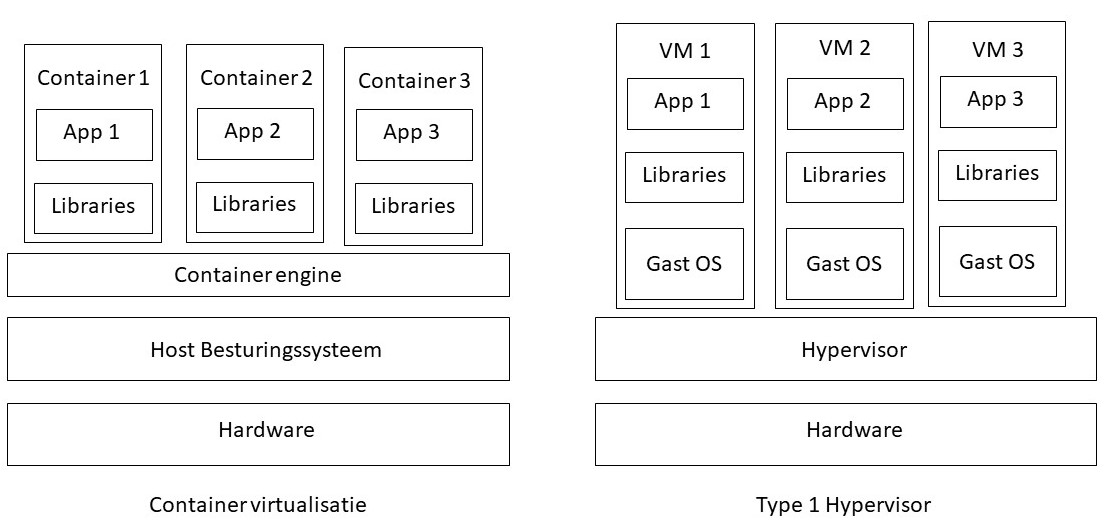
\includegraphics[width=\linewidth]{img/containerVShyper.jpg}
    \caption[Vergelijking container virtualisatie en type 1 hypervisor]{Een vergelijking in werking tussen container virtualisatie en een type 1 hypervisor voor het draaien van apps.}
    \label{fig:containerVShypervisor}
    \centering
\end{figure}

\subsection{Performantie verschillen}
Een vergelijkende studie tussen Containers en virtuele machine gebaseerde virtualisatie\autocite{Yadav2018} haalt aan dat de verschillende manieren van virtualisatie elk hun voordelen en nadelen hebben en dat het afhangt van de noden van de huidige situatie. Dit onderzoek haalt enkel voordelen aan die containers hebben ten opzichte van VM’s zoals: minder nood aan geheugen ruimte, snellere boot-up en hogere draagbaarheid van containers. Maar haalt ook aan de beveiliging bij containers moeilijker is doordat containers direct de host kernel en hardware aanspreken. In een Cloud omgeving zullen zowel VM’s als container virtualisatie hun plaats hebben. Zo zijn VM’s beter geschikt voor Interface as a Service Cloud solution of situaties waar beveiliging van zeer hoog belang is. Terwijl Containers meer toepasbaar is voor Software as a Service.

Een gelijkaardige studie door \textcite{Eder2016} komt tot gelijkaardige conclusies. VM’s en hypervisors zijn een extra laag beveiliging bij virtualisatie. Containers hebben het voordeel van sneller en eenvoudiger te zijn waardoor ze zeer toepasbaar zijn in de cloud omgeving.

Een onderzoek van \textcite{Abdullah2019} heeft vooral gezocht naar de verschillen in opschalen van Multi-level applicaties in een container of VM gebaseerd netwerk. Zij concludeerden dat container based virtualisatie beter is om toenemende vraag aan te kunnen.


\section{Software aanbieders}
In dit deel komen verschillende software pakketten en aanbieders van software voor container virtualisatie aan bod. Hiervoor wordt eerst uitgelegd hoe er een standaard voor containers gedefinieerd werd. Gevolgd door software voor runtimes, engines, container types en orchestration.  Hierna de komen de aanbieders van platformen voor het hosten en delen van container images. Ten slotte enkele grote Cloud service providers en hun ondersteuning voor containers in hun Cloud omgeving.


\subsection{Open Container Initiative}
Om de onderlinge werking en overdraagbaarheid tussen alle mogelijke software te waarborgen is het Open container Initiative(OCI)\footnote{\url{https://opencontainers.org/}} tot stand gebracht. Het OCI legt het twee standaarden voor. De eerste standaard is de runtime specificatie voor het draaien van containers. De tweede standaard is voor het bewaren van de image van een container. 


\subsection{Engines en runtimes}
Er bestaan meerdere engines en runtimes voor containers. De meerderheid is voor linux gebaseerde, en daar mee OCI compliant, containers te draaien. Maar er bestaan ook andere soorten containers die ook in dit deel worden besproken.

\paragraph{Docker engine}
De runtime en daemon waarmee Docker werkt heet de Docker engine. De daemon zelf is gebaseerd op Containerd wat hierna besproken wordt. Het werkt via een Command-line-interface (CLI) om zolang dat de daemon draait containers te kunnen starten, aanmaken of verwijderen. Het laat ook toe huidige containers aan te spreken en status op te halen. De Docker engine word voor Mac os en Windows gebundeld met de Docker desktop, een user interface om de werking van de engine te beheren zonder via de CLI  te moeten werken. De Docker engine is dan ook bruikbaar op alle vaak voorkomende besturingssystemen, maar Linux distributies hebben momenteel geen toegang tot de Docker desktop.
\paragraph{Containerd}
Containerd\footnote{\url{https://containerd.io/}} is een industriestandaard runtime om op Linux en Windows systemen containers te draaien. Door Middel van Go programma’s kan Containerd een container image pullen, configureren, opstarten en beëindigen.
\paragraph{Linux containers}
Zoals eerder aangehaald is Linux containers een manier om met containers te werken op Linux. Het vergt veel kennis van de Linux kernel om goed te kunnen gebruiken.  Het omslaat zowel de LXC manier om containers te maken en draaien. Als een uitbreiding van LXC onder de vorm van LXD. LXC is standaard inbegrepen als deel van veel van de Linux distributies.  
\paragraph{CRI-O}
Cri-o\footnote{\url{https://cri-o.io/}} is een engine die zichzelf verkoopt als een lichter alternatief voor de Docker engine.  Via Cri-o kan op een Linux besturingssysteem via de command line gewerkt worden om eender welk OCI compliant image en runtime software te beheren via Kubernetes.
\paragraph{Podman}
Podman\footnote{\url{https://podman.io/}} is een CLI om Linux containers te creëren, draaien en stoppen op een Linux systeem. Het lijkt doelbewust veel op Docker maar heeft een paar verschillen. zo werkt het zonder een deamon die beheerd moet worden voor het uitvoeren van containers, ook heeft het ingebouwde ondersteuning om meerdere  containers samen te bundelen in een pod en deze in het geheel te beheren..
\paragraph{Windows containers}
Windows Containers\footnote{\url{https://docs.microsoft.com/en-us/virtualization/windowscontainers/about/}} is een specifieke runtime om Windows gebaseerde containers uit te voeren. Het heeft geen eigen engine en berust op integratie met Docker engine en de Docker desktop voor de verdere functionaliteiten. Het draaien van Windows containers is mogelijk op de Server, Enterprise of Education edities van Windows.
\paragraph{Pouch containers}
Pouch containers\footnote{\url{https://pouchcontainer.io/}} is een open source engine voor Linux containers gestart door de Alibaba Group\footnote{\url{https://www.alibabagroup.com/en/global/home}}. Het ondersteunt Linux als besturingssysteem en werkt via een CLI. Het is ook OCI compliant. De laatste stabiele release ten tijden van dit onderzoek was in juni 2019.
\paragraph{Kata containers}
Kata containers\footnote{\url{https://katacontainers.io/}} combineert de beveiligingen voordelen van VM met de draagbaarheid van containers. Zo heeft het ook zijn eigen indeling voor container images.  Het is een open source runtime en berust op een andere engine voor de engine functionaliteiten zoals CRI-O en Containerd. Het kan gebruikt worden op vele Linux distributies.
\paragraph{Andere engine opties}
De volgende opties voor runtimes of engines zijn niet meer goed ondersteunt.
\begin{itemize}
    \item Open vz\footnote{\url{https://openvz.org/}}: Een open source benadering om in Linux zowel containers als virtuele machines te draaien, weinig activiteit sinds 2015.
    \item Rkt\footnote{\url{https://www.openshift.com/learn/topics/rkt}}: Een engine voor linux containers dat na een RedHat acquisitie niet meer ondersteunt wordt, laatste release was 2018.
    \item Balena engine\footnote{\url{https://github.com/balena-os/balena-engine}}: Een specifieke engine voor Internet of Things toepassingen met een laaste release in December 2019.
    \item Flockport\footnote{\url{https://www.flockport.com/}}: Een open source engine met ook wat orchestrion functionaliteiten voor enkele van de meest voorkomende Linux distributies. De open source is niet terug te vinden en heeft bijna geen activiteit meer op de officiële website sinds 2019.ten tijden van dit onderzoek.
\end{itemize}


\subsection{Orchestrion}
Orchestration is een belangrijk deel van de Cloud mogelijkheden van heeft ook verschillende aanbieders van software om dit te organiseren, sommige orchestration software is specifiek voor containers, maar andere laten ook toe om de container orchestration te bundelen met de orchestration voor andere processen zoals klassieke VMs. Voor containers is Kubernetes het meest gekende orchestrations software en volgens onderzoek van \textcite{Truyen2019}, ook de software meet de meeste features.  
\paragraph{Docker compose en Swarm}
Docker Compose is een eerste deel van orchestration die deel uitmaakt van Dockers totaalpakket. Het staat in voor het regelen van applicaties die uit meerdere delen bestaan die elk in een eigen container draaien zolang ze behoren tot één Docker engine. Een voorbeeld hiervan is een webapplicatie zoals Wordpress met een aparte container voor de SQL-databank.  Docker Compose laat een gebruiker toe om via een YAML-file meerdere containers aan elkaar te verbinden en ze later gezamenlijk op te starten en stoppen.

Docker Swarm is het orchestrion gedeelte om over meerdere aparte instanties van Docker engines te werken en werkt ook via een CLI. Hierbij wordt elke instantie van een Docker engine beschouwd als een node binnen de swarm. Er bestaan 2 soorten nodes binnen en Docker Swarm. Manager nodes staan in voor het beheren en delegeren van taken binnen een swarm. De worker nodes voeren de takken uitgestuurd door een managers uit. Standaard is een manager ook een worker maar dit kan uitgezet worden. Om een swarm te hebben moet een engine instantie de swarm initiëren en andere eventuele engines zichzelf toevoegen. Via een manager node kunnen de orchestration instellingen die dan gepropageerd worden over de rest van de manager nodes en uitgevoerd door de worker nodes.
\paragraph{Kubernetes}
Kubernetes\footnote{\url{https://kubernetes.io/}} is een open source orchestration software die container orchestrion toelaat onafhankelijk van de container runtime zolang het de Kubernetes CRI implementeert. Het werkt met pods,  sets van bij elkaar horende containers, die behoren tot een fysieke of virtuele machine die de mogelijkheid heeft om de pods te draaien. Elke van deze machines wordt een node genoemd. Elke node krijgt een kublet die instaat voor het organiseren van het draaien van de pods binnen een node. Daarnaast krijgt ook elke node een proxy om te communiceren met een control plane. De control plane beheert alle nodes in de cluster en kan op één machine staan of ook gedistribueerd zijn.  Standaard werkt kubernetes via command line maar heeft de mogelijkheid om dashboard ui bij te instaleren.
\paragraph{Red hat Openshift}
Openshift\footnote{\url{https://www.openshift.com/}} is Red Hat’s uitbreiding en extensie van de kubernetes software om dienst te doen als orchestration software. Openshift wilt toelaten om orchestration gelijktijdig te regelen over eigen on premise servers en servers die van een Cloud hosting provider worden benut. Hier blijft niet enkel bij eigen servers en één Cloud service, het laat zelfs toe om de orchestration te doen over meerde Cloud serviceproviders.
\paragraph{Nomad}
Nomad\footnote{\url{https://www.nomadproject.io/}} is een Enterprise gefocuste orchestration software aangeboden door Hashi Corp dat ook gemengde orchestration op grote schaal toelaat. Het verkoopt zichzelf als een manier om met containers om te gaan als vervanging of aanvulling van Kubernetes. Naast een CLI komt het standaard ook met een web User interface om orchestration te regelen.
\paragraph{Apache Mesos}
Mesos\footnote{\url{http://mesos.apache.org/}} is een orchestrion framework van apache die grotere schaal orchestrion toelaat. Naast containers heeft het ook ondersteuning om Virtuele machines te beheren. Het maakt een abstractie van de kernel over meerdere machine heen om zo in een server context orchestrion te regelen.
\paragraph{DC/OS}
De Distributed Cloud Operating System\footnote{\url{https://dcos.io/}} is een open source besturingssysteem dat gebaseerd is op apache Mesos om via een singuliere interface meerdere machines te bereiken. Om zo orchestration van containers en meer over de meerdere machines toe te laten.
\subsection{Image repositories}
Om container images te kunnen delen met andere zijn er repositories die deze remote kunnen bewaren. Naast de drie die in dit deel besproken worden, bieden Cloud providers ook hun eigen repositories aan voor intern gebruik binnen hun Cloud omgeving.
\paragraph{Docker Hub}
De Docker Hub\footnote{\url{https://hub.docker.com/}} is de grootste en meest gekende repository voor container images. Het heeft zo een grote bibliotheek aan images. Veel vaak gebruikte images worden dan ook gehost op de Docker Hub en Docker help ook bij het erkennen van officiële images. Voor het hosten van eigen images op de Docker zijn publieke images gratis. Een gratis account heeft de mogelijk om 1 repository private te zetten. De limieten op het pullen of pushen van images die tot een gratis account behoren zijn maximaal 100 anonieme en maximaal 200 ingelogde per zes uur. 
\paragraph{GitHub Container Registry}
GitHub werkt aan een functionaliteit om als gebruiker of onderneming op GitHub container images te bewaren genaamd de  GitHub Container Registry\footnote{\url{https://docs.github.com/en/packages/guides/about-github-container-registry}}. Het ondersteund zowel Docker’s eigen images als OCI images. Het is een deel van GitHub’s packages en is momenteel nog in bèta. De container registry wijkt af van de GitHub packages in mate dat de container images niet gekoppeld moeten zijn met een github repository. Hierdoor zijn de toegangsrechten van de images onafhankelijk van eventuele repositories waartoe ze behoren en kunnen deze afzonderlijk ingesteld worden. Bijkomend is het mogelijk om een publiek gedeelde container image anoniem te downloaden wat met gewone packages niet toegestaan is. Tijdens de bèta is het gebruik van de container registry volledig gratis. Eens het uit beta is zal de container registry samen met de rest van de GitHub packages gefactureerd woorden. Namelijk publieke bestanden gratis, en een limiet op bestands grootte en data overdracht voor private images.
\paragraph{GitLab Container Registery}
De GitLab Container Registry\footnote{\url{https://docs.gitlab.com/ee/user/packages/container_registry/}} is gebaseerd op de Dockers Container Registery. Het laat toe om per Gitlab project een locatie voor container images te alloceren. Voor het ophalen en uploaden van images werkt het met de met de het met de Gitlab CLI. Het laat ook private en publieke images toe, in de vorm van overerving van de toegankelijkheid van het project waartoe de registry behoort. 


\subsection{Cloud hosting en services}
De grootte Cloud hosting en service providers bieden elk ondersteuning voor containers aan en hebben niet veel verschillen.
\paragraph{Amazon AWS}
Als deel van Amazon’s Cloud services biedt het via AWS\footnote{\url{https://aws.amazon.com/}} toegang tot 3 Container verwante services. De eerste is Het Amazon Elastic Container Registry (ECR). Het ECR is specifiek voor het bewaren van container images en de toegang configuratie tot de registry. De tweede is het Amazon Elastic Container Service (ECS). Het ECS staat in voor het uitvoeren van container gebaseerde applicaties op Amazon’s webhosting services aan de hand van Amazon’s eigen manier van orchestrion. En de derde is het Amazon Elastic Kubernetes Service (EKS). Dit laat ook toe om container gebaseerde applicaties te draaien maar dan met een Kubernetes gebaseerde aanpak voor het beheren en opschalen van de containers. Naast de 3 specifieke services is het ook mogelijk om een container host te installeren op de generische Elastic Compute Cloud webhosting van AWS.
\paragraph{Microsoft Azure}
Microsoft’s Azure\footnote{\url{https://azure.microsoft.com/}} heeft ook ondersteuning voor containers met 3 primaire services die nauw lijken op de services van Amazon. Eerst is er de Azure Container Registry (ACR). Het ACR is de container registry methode van Azure. De tweede is de Azure Container Instances (ACI). Het ACI is analoog aan  Amazon’s ECS voor het uitvoeren van containers en de bijhorende orchestration. Ten slotte biedt Azure ook Azure Kubernetes Services (AKS) aan. Het AKS is dan de manier om op Azure de Kubernetes gebaseerde aanpak te gebruiken. Ook hier is er naast deze servies mogelijk om containers te hosten om Azure’s Web Apps hosting service.
\paragraph{Google Cloud}
Google’s Cloud\footnote{\url{https://cloud.google.com/}} zet de trend verder met hun Google Container Registry (GCR), Google Cloud Run (GCR) en Google Kubernetes Service (GKE). Deze 3 services zijn elk analoog aan hun equivalenten in AWS en Azure. Ook in Google's Cloud is er de mogelijkheid om een container host te installeren om de algemene hosting service Google Compute Engine.
\paragraph{IBM Cloud}
De IBM Cloud\footnote{\url{https://www.ibm.com/cloud}} biedt ook ondersteuning voor containers. Zo heeft het ook een container registry en een kubernetes gebaseerde container hosting service.
\paragraph{Red Hat OpenStack}
Voor het werken over verschillende Cloud service providers met Openshift zijn er momenteel 4 Cloud providers die integratie met OpenShift hebben. Azure, IMB en AWS hebben een specifieke service voor OpenShift op hun systeem. Verder bieden Google Cloud en AWS de mogelijkheid om hun hardware te gebruiken om een niet direct met de provider gekoppelde instantie te hosten.



